\section{Browser Security Warnings and HTTPS Errors}
%����Ҫ��дһ���ܽ���ܵĻ�
\subsection{Browser Security Warnings}
Browser uses security warnings to protect users by alerting them to network attacks. 
    According to different levels of risk, 
    Browser presents different connection security states in order to maximize security and minimize side effects of user experience. We describe security warnings of major browsers.

\subsubsection{Risk Level A: Low-risk warnings}
In this scenario, a passive security indicator indicates minor HTTPS errors by removing lock icon, changing lock icon��s color, providing textual information, or by other means without interrupting the users' browsing. This kind of warning is only shown on the status bar other than the full screen.
\begin{figure}[htbp]
\centerline{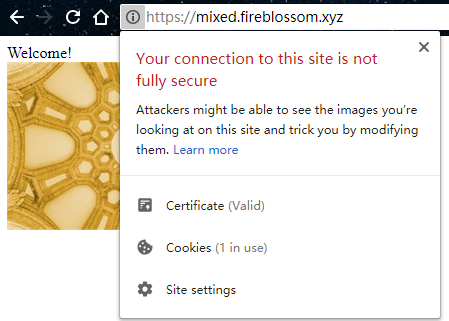
\includegraphics[height=3cm,width=7cm]{Figure/fig1.png}}
\caption{low-risk warning in chrome.}
\label{fig}
\end{figure}

\subsubsection{Risk Level B: Medium-risk warnings that can be bypassed}
Bypassable HTTPS security warnings are the most common type of browser warning. Browsers use bypassable HTTPS security warning to treat the vast majority of HTTPS errors.
\begin{figure}[htbp]
\centerline{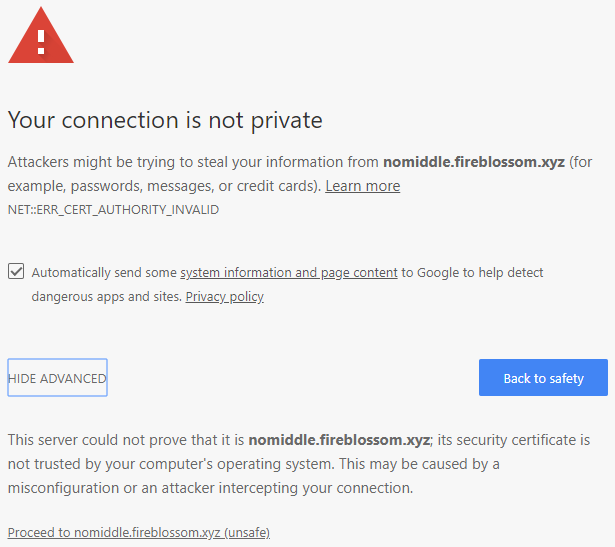
\includegraphics[height=3cm,width=7cm]{Figure/fig2.png}}
\caption{medium-risk warning in chrome.}
\label{fig}
\end{figure}

In this scenario, if there is an HTTPS error, the browser will stop the page load and display a full-screen HTTPS security warning. 
    Typically,
    Users can choose to close the webpage or click through the warning by clicking on a button. 
    Although the HTTP(s) traffic we captured through Fiddler[ https://www.telerik.com/fiddler] shows the web page is not transmitted in plain text, 
    clicking through the warning may allow an actual man-in-the-middle attack to proceed.

\subsubsection{Risk Level C: High-risk warnings that cannot be bypassed}
As a worst case scenario, 
    the browser will prevent uses from continuing to browse the website by showing a full-screen security warning that the users cannot bypass.
\begin{figure}[htbp]
\centerline{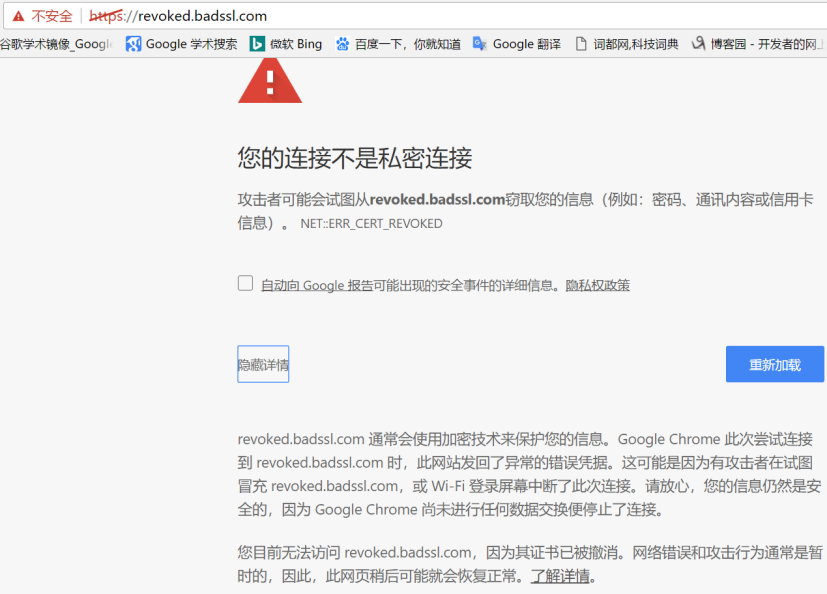
\includegraphics[height=3cm,width=7cm]{Figure/fig3.png}}
\caption{high-risk warning in chrome.}
\label{fig}
\end{figure}
Major browsers have small differences in warning appearances.
    For example, 
    chrome displays a red triangle, but IE shows a red shield to imply danger.

\subsubsection{Risk Level D: Cannot establish HTTPS connection}
The browser may fail to establish a HTTPS connection to the server for unsupported TLS version, cipher mismatch, or other reasons. In this scenario, the browser cannot obtain certificates from the web server, let alone certificate validation, so the TLS handshake error is not discussed in this paper.
\begin{figure}[htbp]
\centerline{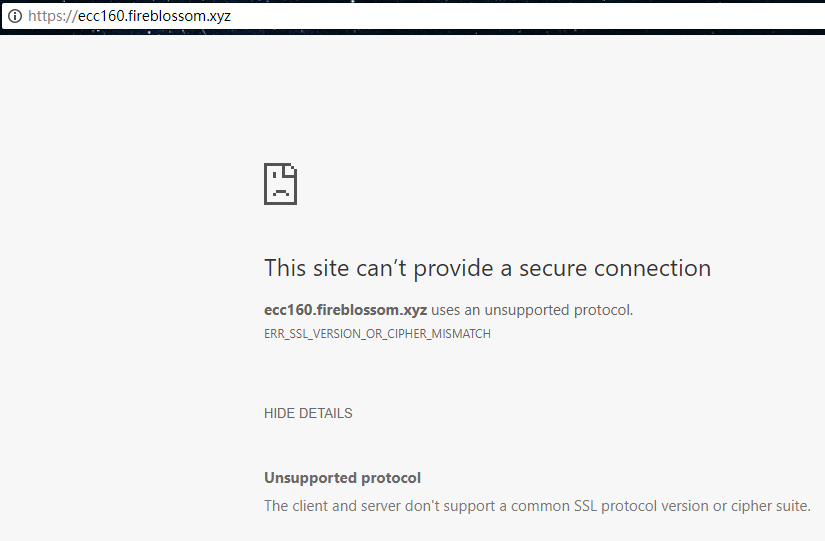
\includegraphics[height=3cm,width=7cm]{Figure/fig4.png}}%��ͼ��Ҫ�ٵ�����������
\caption{Cannot establish HTTPS connection in chrome.}
\label{fig}
\end{figure}
